\chapter{Three-Tier Defense-in-Depth Implementation}
\label{chap:defense_layers}

This chapter analyzes the concrete engineering implementation across the three progressive inspection layers: the perimeter reverse proxy, the role-aware API Gateway, and the inline payload inspector IDS.

\begin{figure}[htbp]
\centering
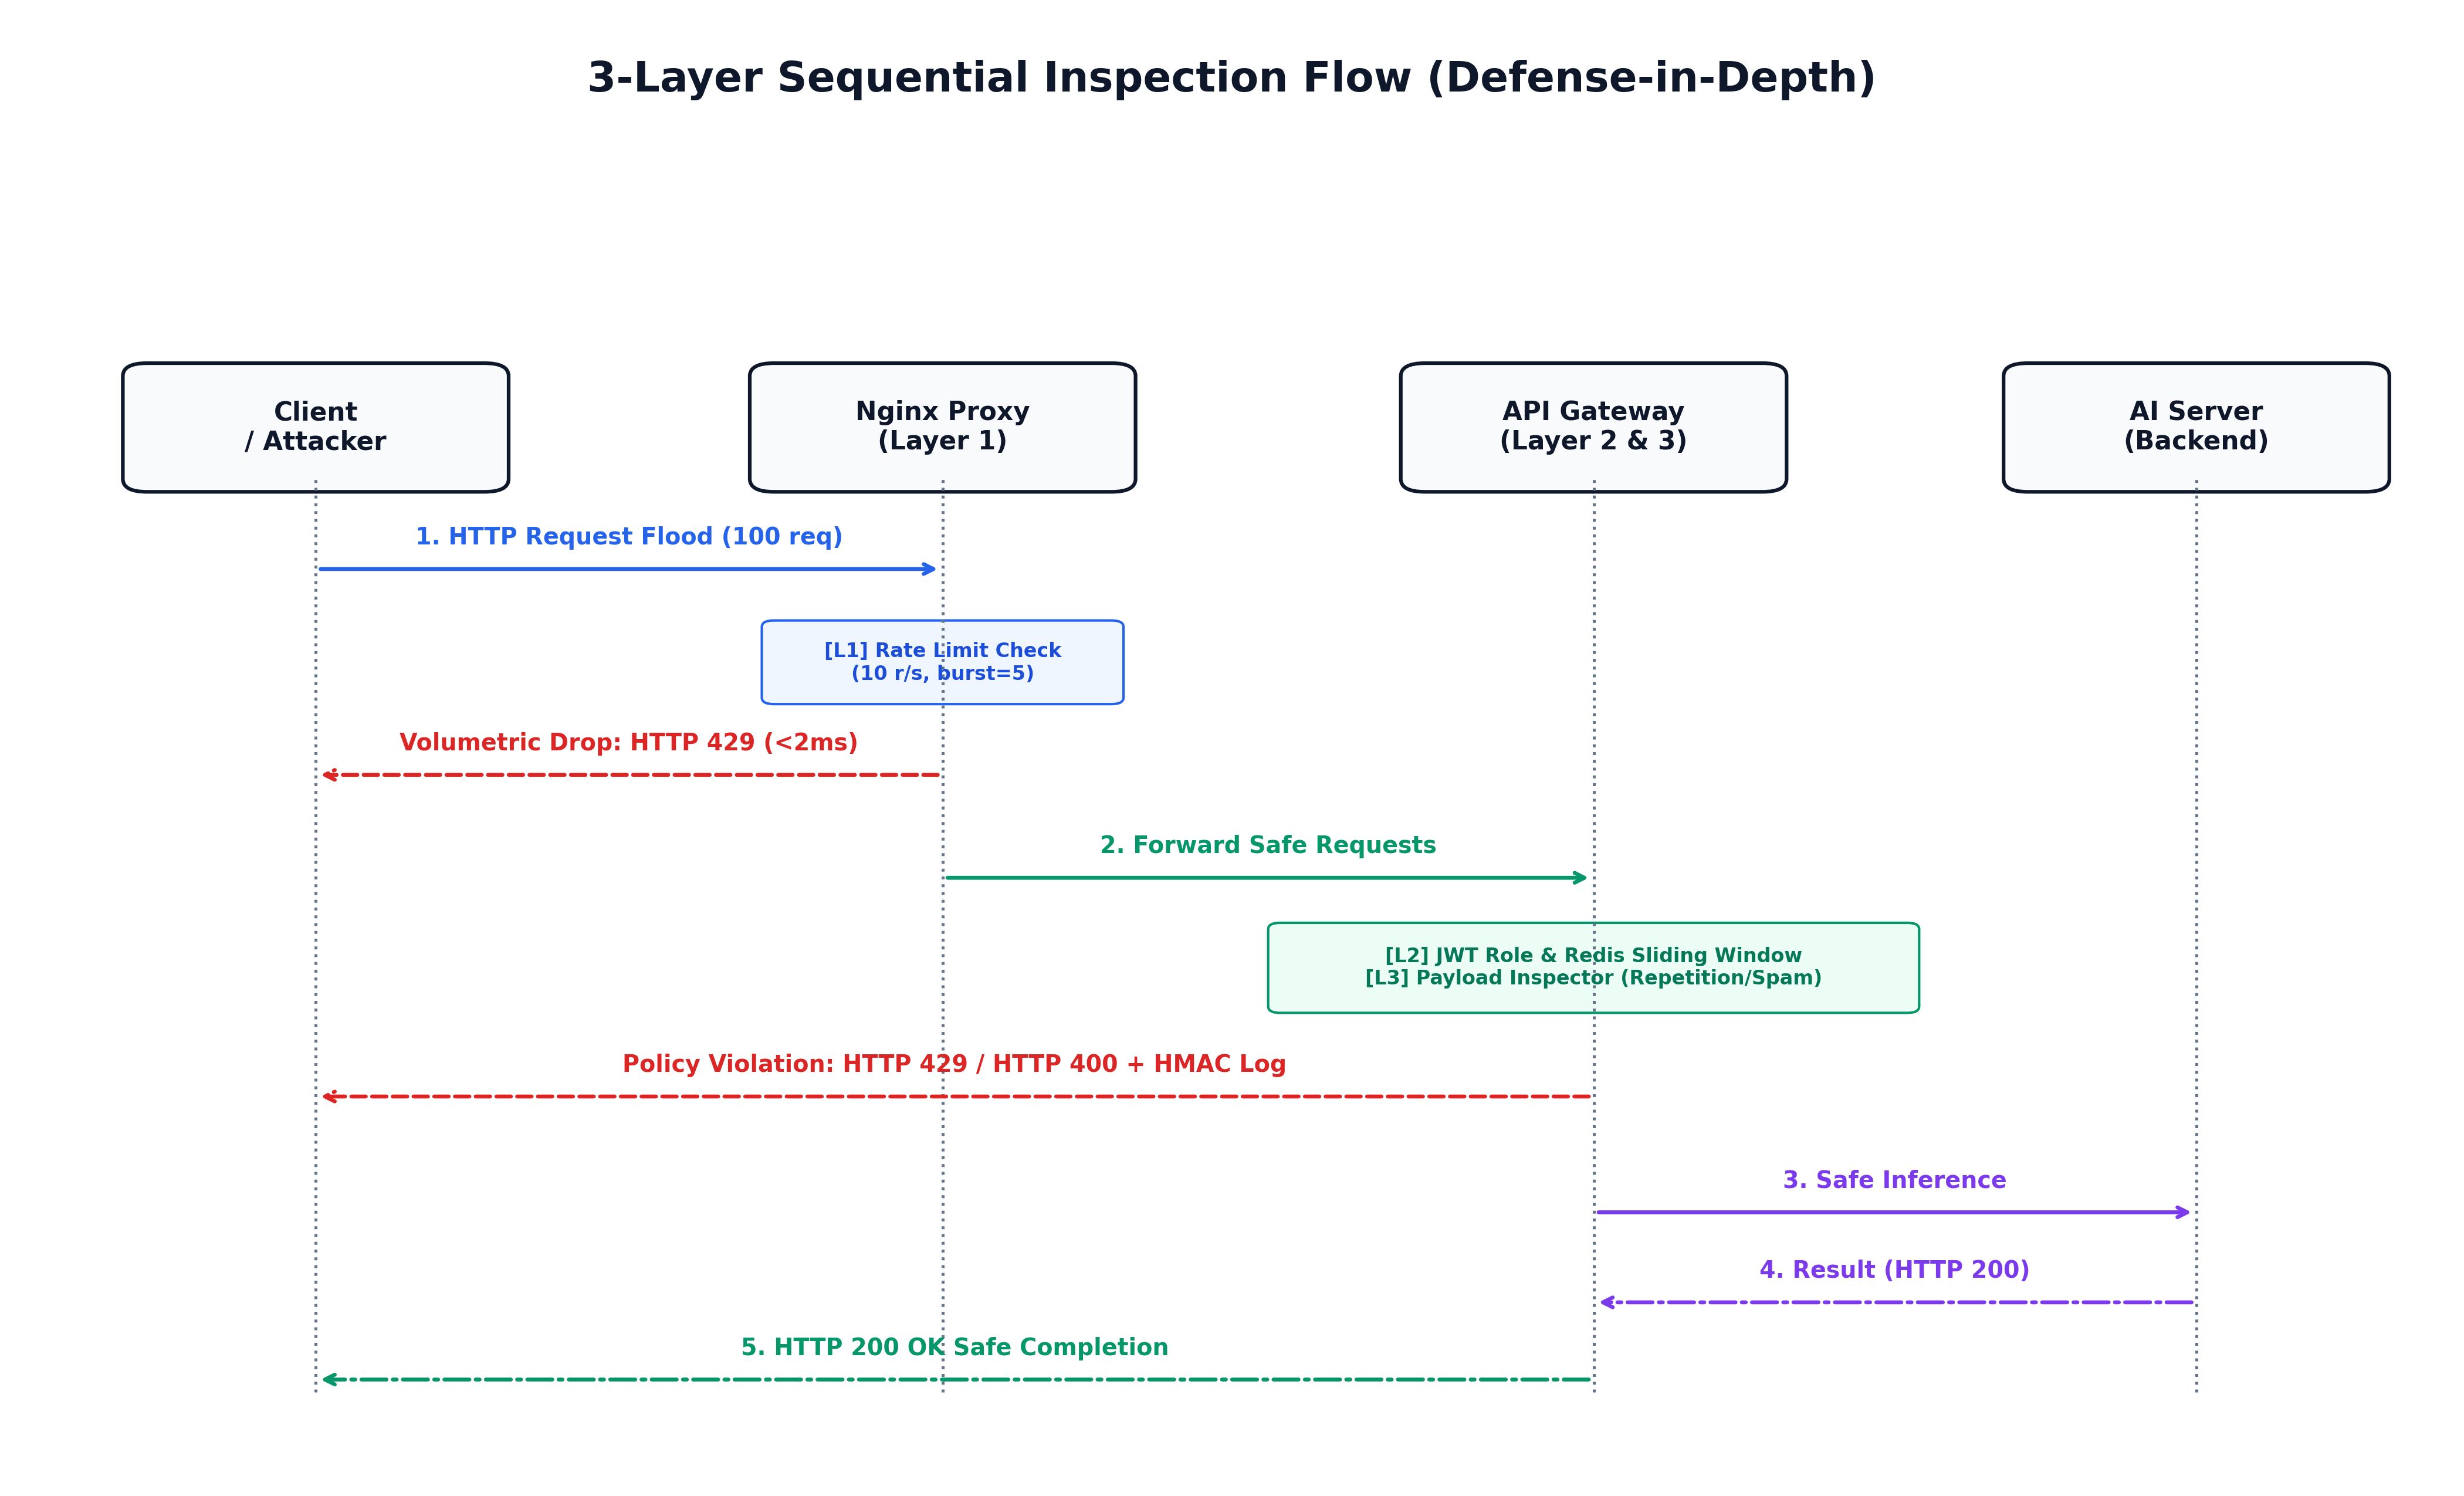
\includegraphics[width=0.95\textwidth]{figures/sequence_defense_layers.png}
\caption{Sequential Multi-Tier Inspection Workflow (Defense-in-Depth).}
\label{fig:sequence_defense_layers}
\end{figure}

As depicted in Figure~\ref{fig:sequence_defense_layers}, requests progress through sequential checkpoints. A failure at any tier triggers an immediate short-circuit termination.

\section{Tier 1: Perimeter Volumetric Rate Limiting (Nginx)}
The first line of defense is deployed on Nginx in the DMZ. Utilizing \texttt{ngx\_http\_limit\_req\_module}, it throttles incoming HTTP request volume based on client IP:

\begin{lstlisting}[language=c, caption={Nginx Ingress Configuration with Memory Rate Limit Zone}]
http {
    limit_req_zone $binary_remote_addr zone=api_limit_zone:10m rate=10r/s;

    server {
        listen 80;

        location /api/v1/ {
            limit_req zone=api_limit_zone burst=5 nodelay;
            limit_req_status 429;
            proxy_pass http://ai-api-gateway:8000/;
        }
    }
}
\end{lstlisting}

\begin{itemize}
    \item \textbf{\texttt{\$binary\_remote\_addr}}: Uses 4-byte binary IPv4 representations, tracking up to 160,000 distinct IP addresses in a compact 10MB memory zone.
    \item \textbf{\texttt{burst=5 nodelay}}: Absorbs brief legitimate spikes while instantly rejecting volumetric bursts exceeding 10 req/s with \texttt{HTTP 429} in $<2\,\text{ms}$.
\end{itemize}

\section{Tier 2: Role-Based Access Control and Atomic Sliding Window (FastAPI + Redis)}
Legitimate requests passing Tier 1 reach the asynchronous FastAPI Gateway (ASGI Uvicorn \cite{fastapi}). 

\subsection{JWT Cryptographic Authentication}
Clients authenticate via standard Bearer tokens conforming to RFC 7519 \cite{rfc7519}. The gateway decodes the claims and validates identity and user roles (\texttt{guest}, \texttt{employee}, \texttt{admin}). Unauthenticated or forged tokens trigger an immediate \texttt{HTTP 401 Unauthorized}.

\subsection{Atomic Sliding Window Algorithm on Redis ZSET}
To prevent boundary burst flaws inherent in fixed-window limiters, the Gateway enforces a dynamic sliding window backed by Redis Sorted Sets (\texttt{ZSET}) \cite{redis}:
\begin{enumerate}
    \item \textbf{Prune}: Evict timestamps older than $(t_{\text{current}} - W_{\text{window}})$ using \texttt{ZREMRANGEBYSCORE}.
    \item \textbf{Count}: Query active requests in the current window using \texttt{ZCARD}.
    \item \textbf{Admit / Drop}: If count exceeds the role quota ($Q_{\text{guest}}=5$, $Q_{\text{employee}}=60$), return \texttt{HTTP 429}; otherwise, record $t_{\text{current}}$ via \texttt{ZADD}.
\end{enumerate}
All operations are executed atomically in Redis to guarantee concurrency safety under high parallel load.

\section{Tier 3: Inline Payload Inspector IDS Heuristics}
Authenticated requests within quota limits undergo content-level inspection prior to backend dispatch:
\begin{itemize}
    \item \textbf{Input Length Cap}: Enforces a strict maximum bound ($L_{\max}=500$ characters). Prompts exceeding this cap are immediately rejected with \texttt{HTTP 400 Bad Request}, guarding against attention memory explosion.
    \item \textbf{Token Repetition Ratio}: Computes lexical vocabulary diversity:
    \begin{equation}
        \text{Repetition Ratio} = 1.0 - \frac{\text{Count}(\text{Unique Words})}{\text{Count}(\text{Total Words})}
    \end{equation}
    Prompts with a repetition ratio exceeding $0.3$ combined with high token volume trigger a semantic DoS block (\texttt{HTTP 400}).
\end{itemize}

\section{Tamper-Evident Forensic Logging (HMAC-SHA256)}
To ensure non-repudiation and forensic auditability, every security event is recorded as a structured JSON object cryptographically signed using an HMAC-SHA256 hash (RFC 2104 \cite{rfc2104}), guaranteeing tamper detection across centralized log streams.
